\subsection{Distortion and entropy measures}

\begin{figure}
  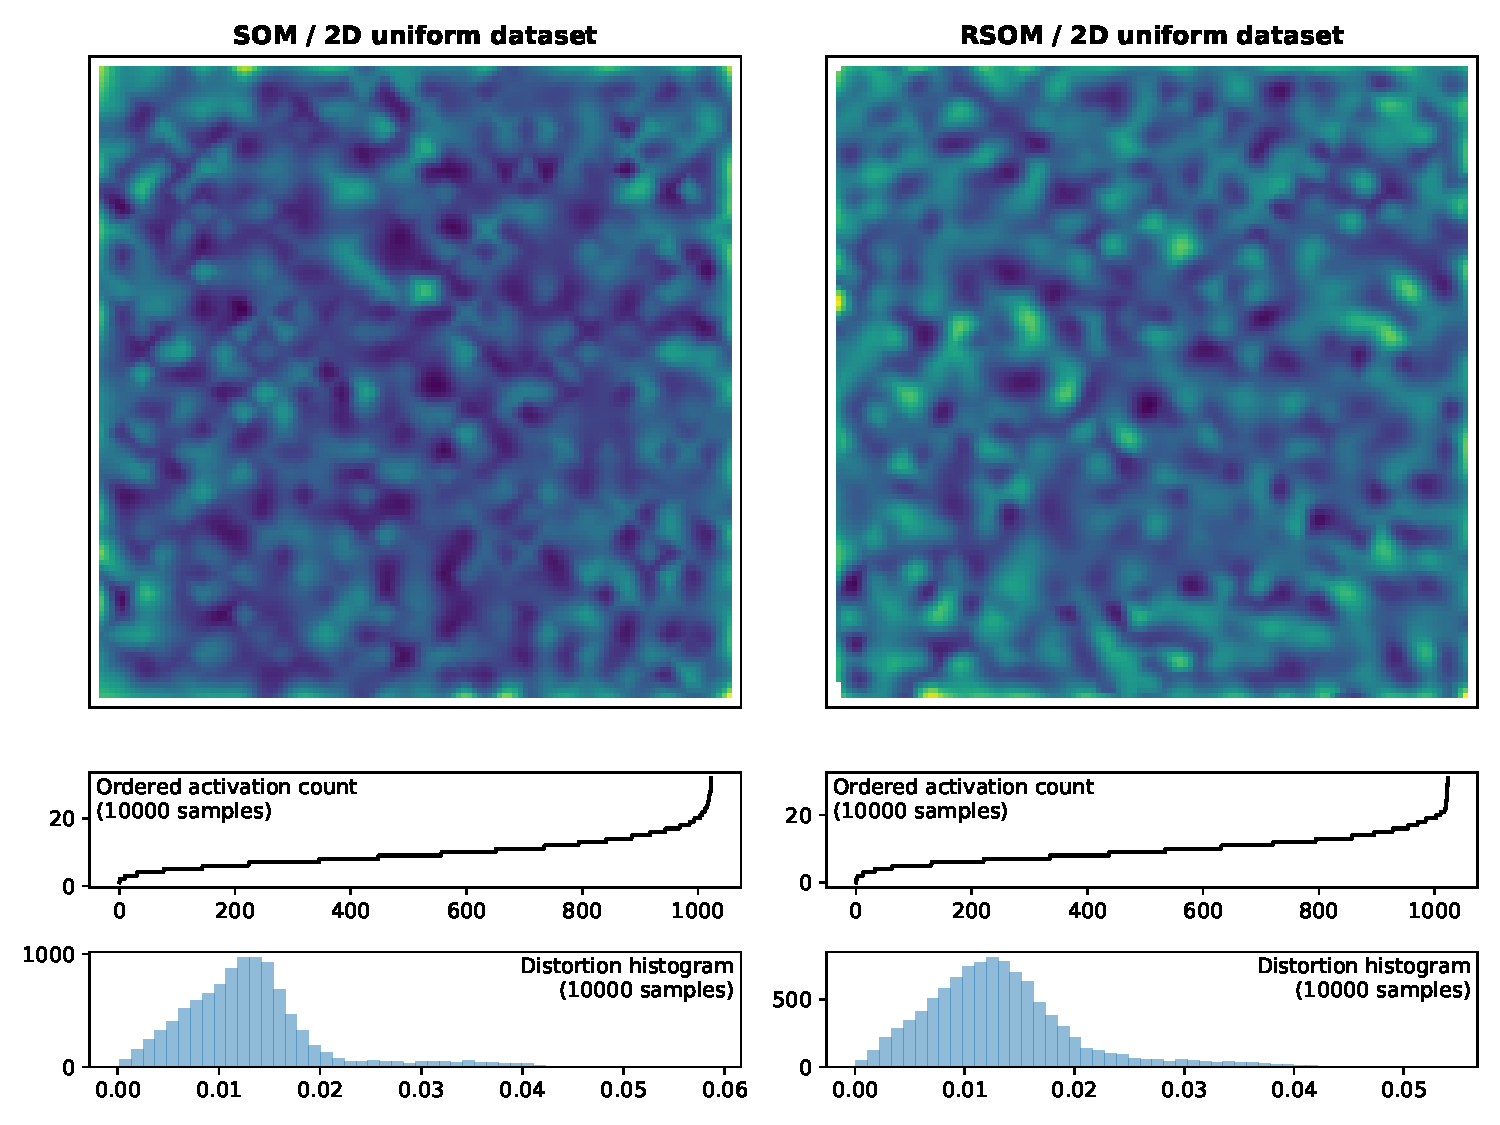
\includegraphics[width=\columnwidth]{experiment-2D-uniform-activation-distortion.pdf}
  \caption{\textbf{Two dimensional uniform dataset (measures)}. Measure of distortion and mean activation over 10,000 samples.}%
\end{figure}

\begin{figure}
  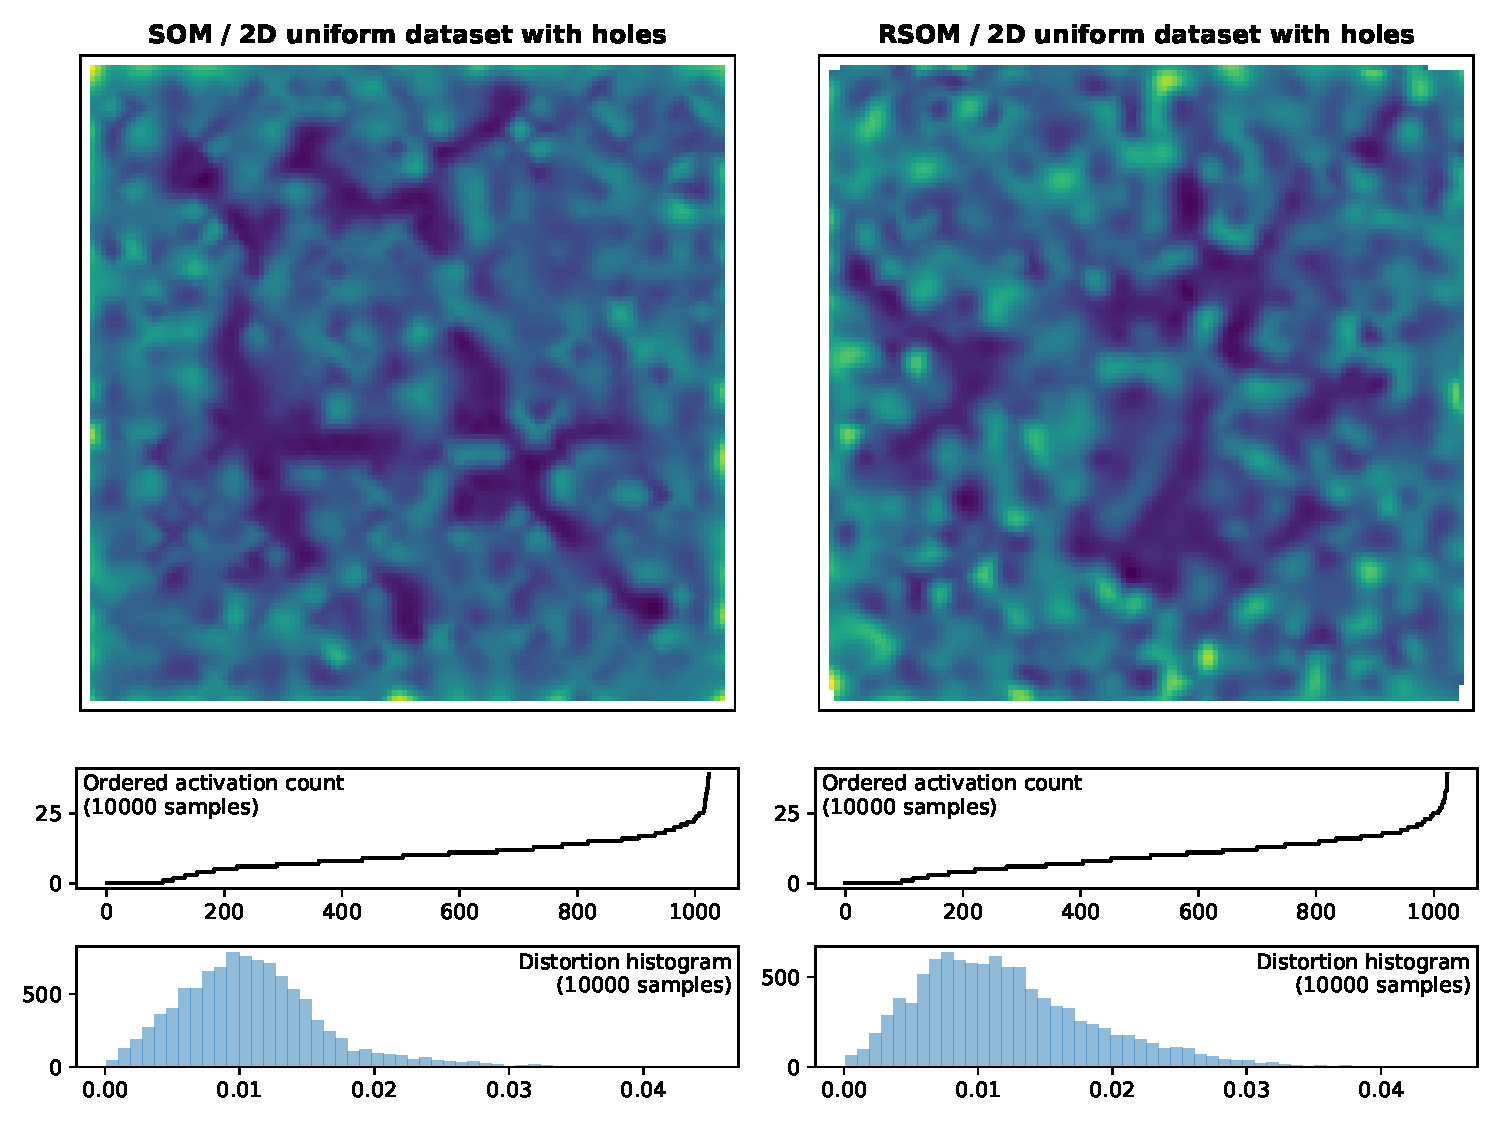
\includegraphics[width=\columnwidth]{experiment-2D-holes-activation-distortion.pdf}
  \caption{\textbf{Two dimensional uniform dataset with holes (measures)}Measure of distortion and mean activation over 10,000 samples.}%
\end{figure}

\begin{figure}
  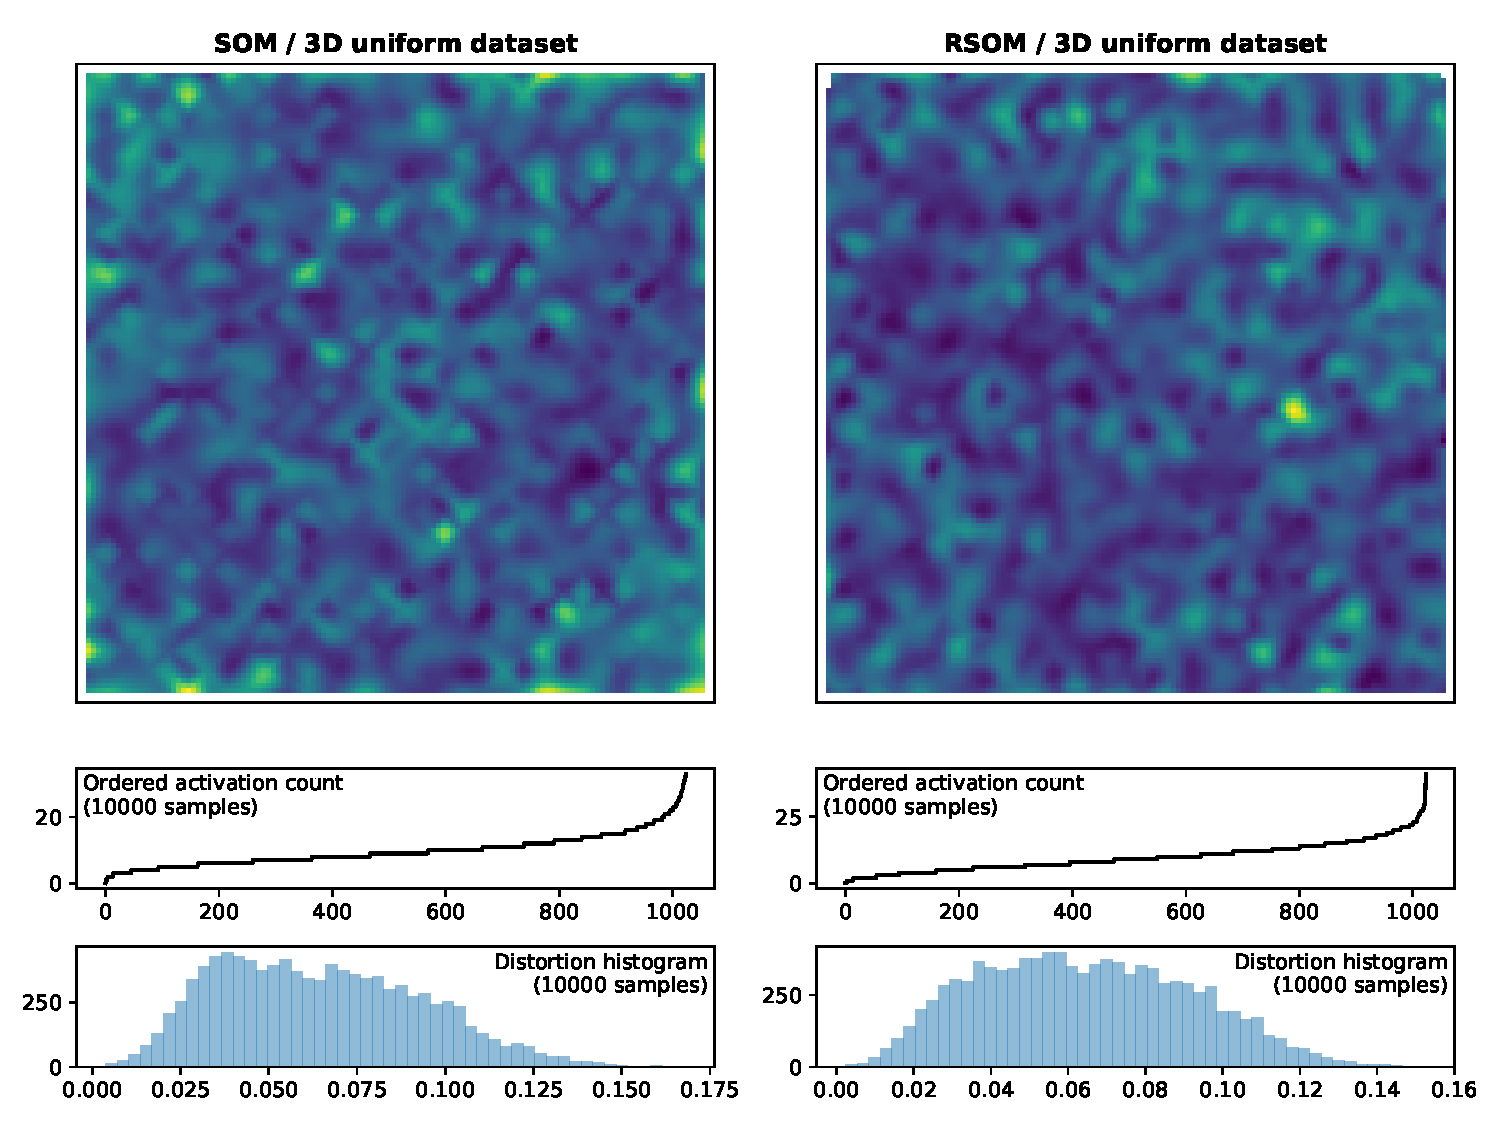
\includegraphics[width=\columnwidth]{experiment-3D-uniform-activation-distortion.pdf}
  \caption{\textbf{Three dimensional uniform dataset (measures)}. Measure of distortion and mean activation over 10,000 samples.}%
\end{figure}

\begin{figure}
  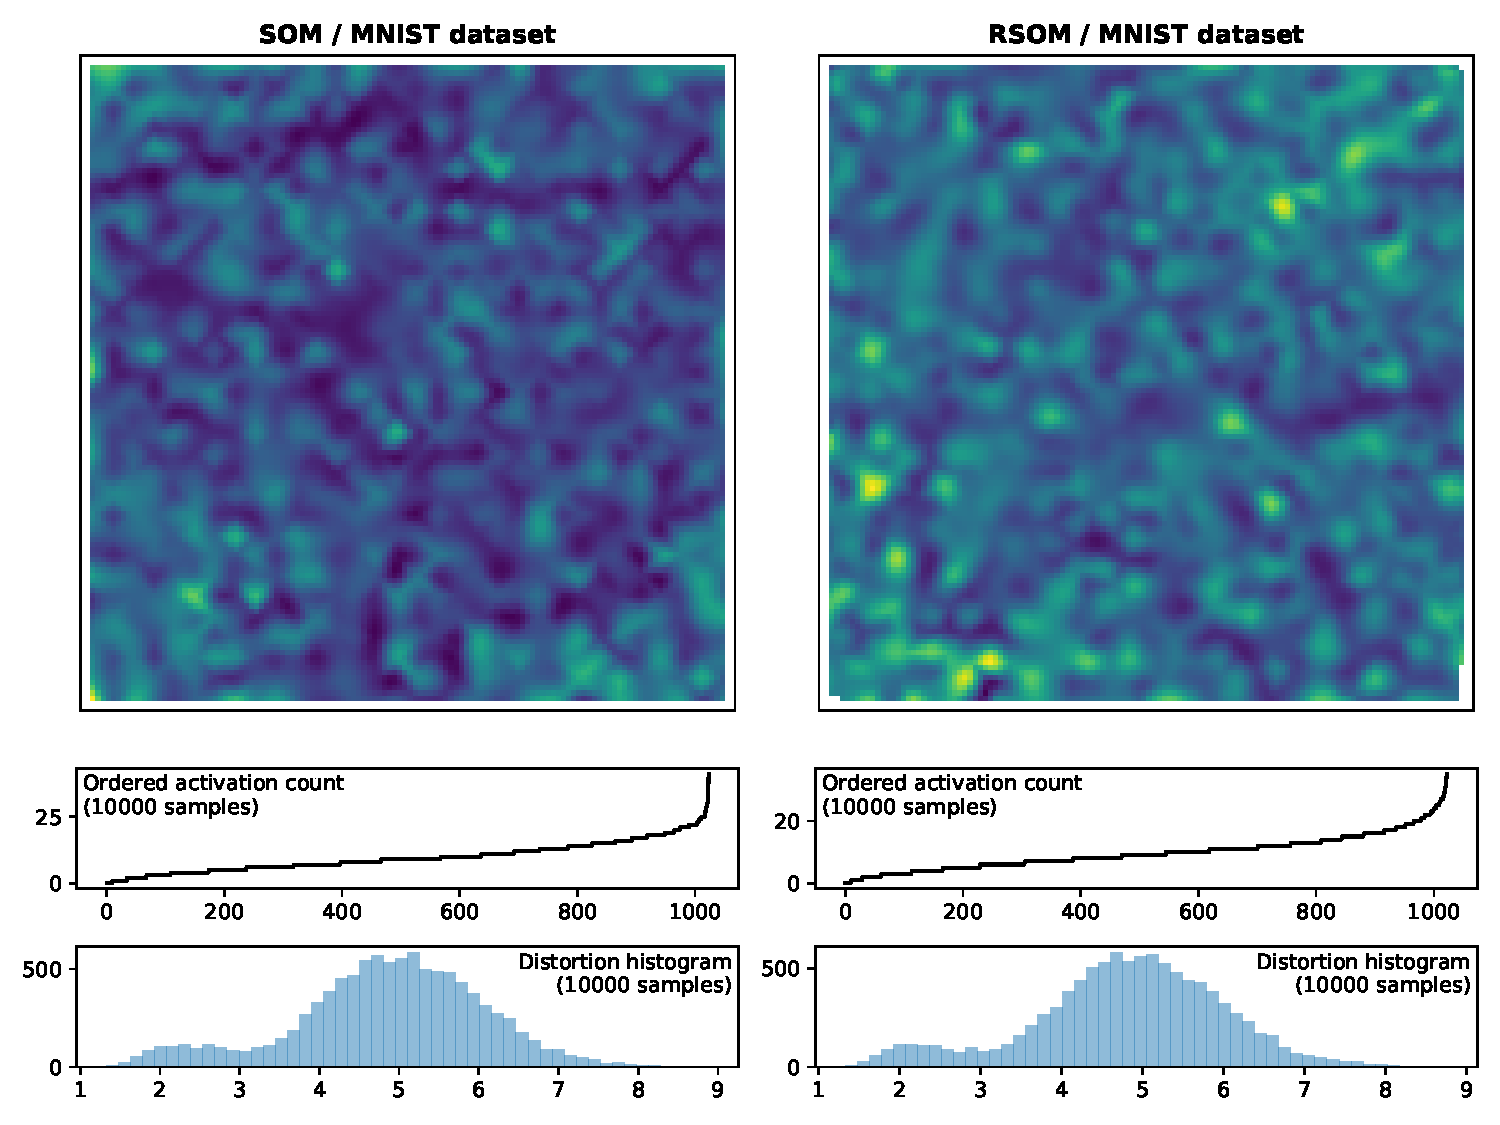
\includegraphics[width=\columnwidth]{experiment-MNIST-activation-distortion.pdf}
  \caption{\textbf{MNIST dataset (measures)}. Measure of distortion and mean activation over 10,000 samples.}%
\end{figure}
